\chapter{Introduction}
\label{c:introduction}

\section{Overview}
\label{section:overview}

This research aims to develop a novel gantry machine to precisely water the soil portion of orchid seedlings, the incidence rate of which will be accordingly decreased due to lower infiltration on leaves. In the previous research of Cartesian watering machines, the entire performance was decreased because of the high time cost to turn the watering valve on and off. It is supposed that the seedling grows symmetrically with two sides of leaves aligned on a straight line. This research installs the watering sprayers on the motion actuators, which are controlled to pass through the seedlings center perpendicular to the leaves' growth direction in order to prevent splashing water from leaves. Three main topics in this research are:

\begin{enumerate}
    \item Pose estimation of 2D Seedling
    \item Trajectory planning of gantry actuator
    \item Prototype implementation of gantry robot 
\end{enumerate}

The seedling pose estimator provides the seedling position and the growth direction of leaves using YOLOv4-tiny and regression of the region of interest (RoI). Then, the trajectory planner will control the linear actuators using the pose of seedlings. Finally, this research completes the prototype of the gantry machine, entitled ``XsY gantry robot'', to implement the proposed methods. Unlike the XY gantry machine, which has a single coordinate system, the XsY gantry robot is a multi-coordinate system that shares the same y-axis. Therefore, the name ``XsY'' means that the robot has multiple x-axes that are controllable, as shown in Fig.\ref{fig:xsymodel}.

\begin{figure}[ht]
    \centering
    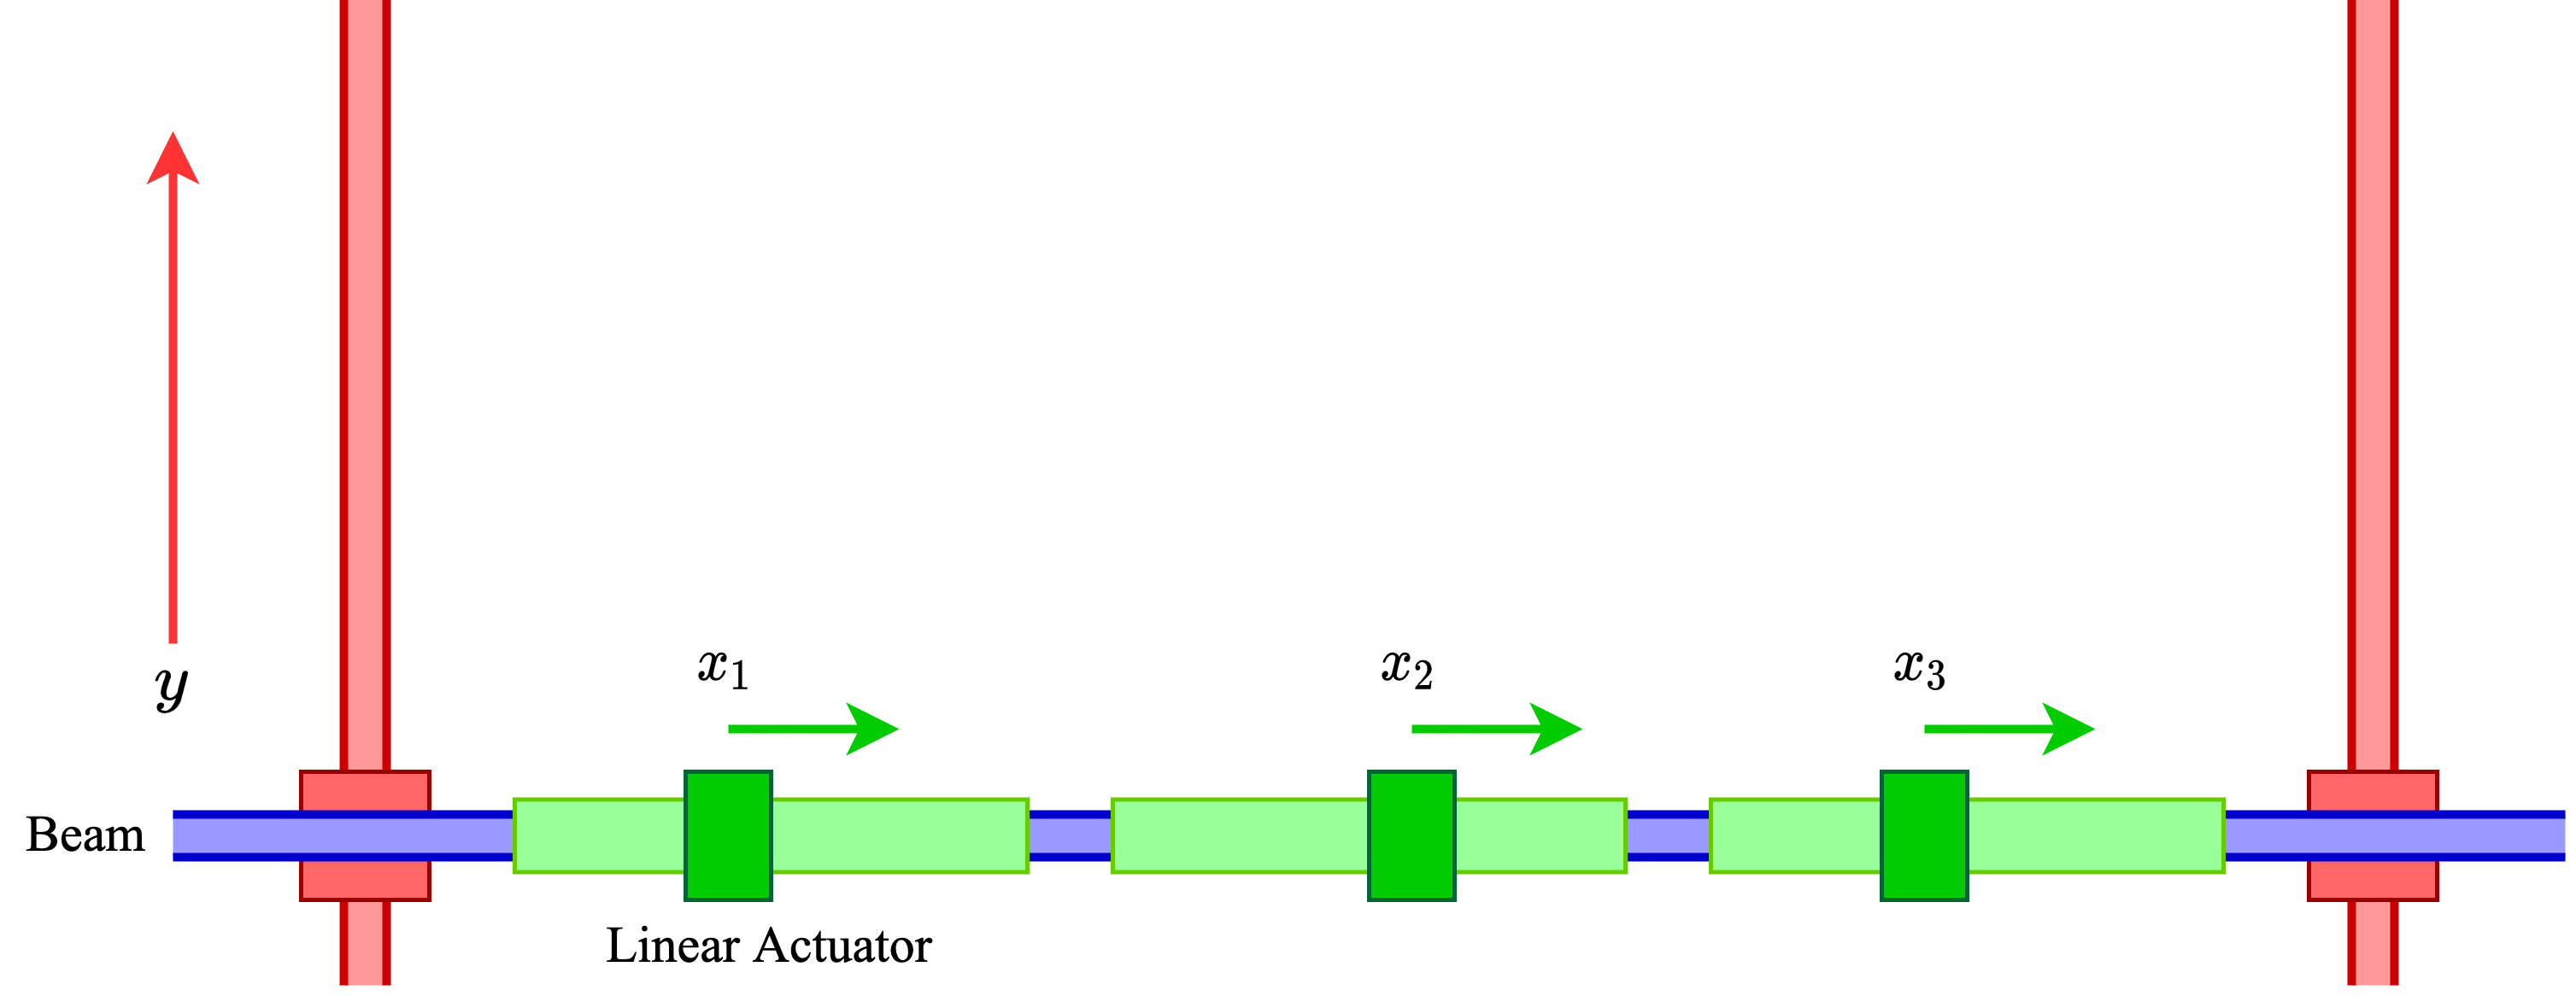
\includegraphics[width=0.7\textwidth]{figsrc/ch01/XsY Gantry.png}
    \caption{XsY gantry model}
    \label{fig:xsymodel}
\end{figure}


To evaluate the performance of this work, two metrics are adopted to determine the performance of the gantry robot: watering success rate and watering speed.

% ===== Check Line V2 2021/08/09
% ===== Check Line V2.1 2021/08/24

\section{Background and Motivation}
\label{section:motivation}

% The importance of agriculture in Taiwan
From the 1960s, Taiwan began to develop floriculture for the purpose of industrial diversification. However, in recent years, Taiwan has encountered severe structural problems: the rapid aging of the agricultural population and the scarcity of young farmers entering the profession. The lack of agricultural population, a significant problem, currently impacts the agriculture of Taiwan, particularly in floriculture. According to the statistical data from The Council of Agriculture in Taiwan\cite{行政院農委會_農業就業人口統計}, the agricultural population was only 550 thousand until March 2020. Furthermore, these farmers' average age is highly old at 62 in 2017\cite{黃柏軒_2018} and will be much older in the future. Due to this challenge, it is an essential mission for Taiwan to develop intelligent and automatic agriculture.

% Orchids
Moreover, as an important plant with a high economic value in Taiwan, the number of orchids reaches up to 15.8 million USD, out of 78\% of the overall exportation of flowers, with exports. In addition, the phalaenopsis (or moth orchids), one of the species of orchids, has even an exporting value of more than 13.9 million USD, 88\% of the total orchids, as shown in Fig.\ref{fig:export-orchid}\cite{行政院農委會_單一農產品進出口量值}.

\begin{figure}[ht]
    \centering
    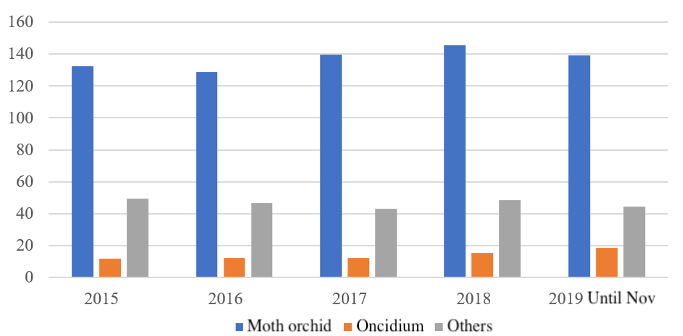
\includegraphics[width=0.8\textwidth]{ch01/export_orchid_en.png}
    \caption{Exporting Value of Orchids In Past Years In Taiwan}
    \label{fig:export-orchid}
\end{figure}

% Automatic system
In the modern greenhouse, companies tend to introduce various automatic systems rather than human power to automate the production process, which can help solve the laboring shortage of agriculture. In most situations, the automatic machine can enhance the product quality and curtail the laboring cost. However, it is still advantageous for humans to tackle some sophisticated tasks. Especially in agriculture, the irregular shapes of plants make it difficult to be treated by machine. Furthermore, despite being designed for automatic watering, seeding, or pollination, earlier research works may only focus on specific species. In this research, the main problem comes from the usage of the watering machine.

% The watering
The watering system plays a critical role in the manufacture of orchids. Plants need to be watered to grow and live; simultaneously, farmers mix the fertilizer and the water to make it easier for plants to absorb the nutrient. Originally, most of the watering tasks are completed by the human. For example, Fig.\ref{fig:HumanWater} demonstrates that the farmer uses a water jet to water the orchid seedlings.

\begin{figure}[ht]
    \centering
    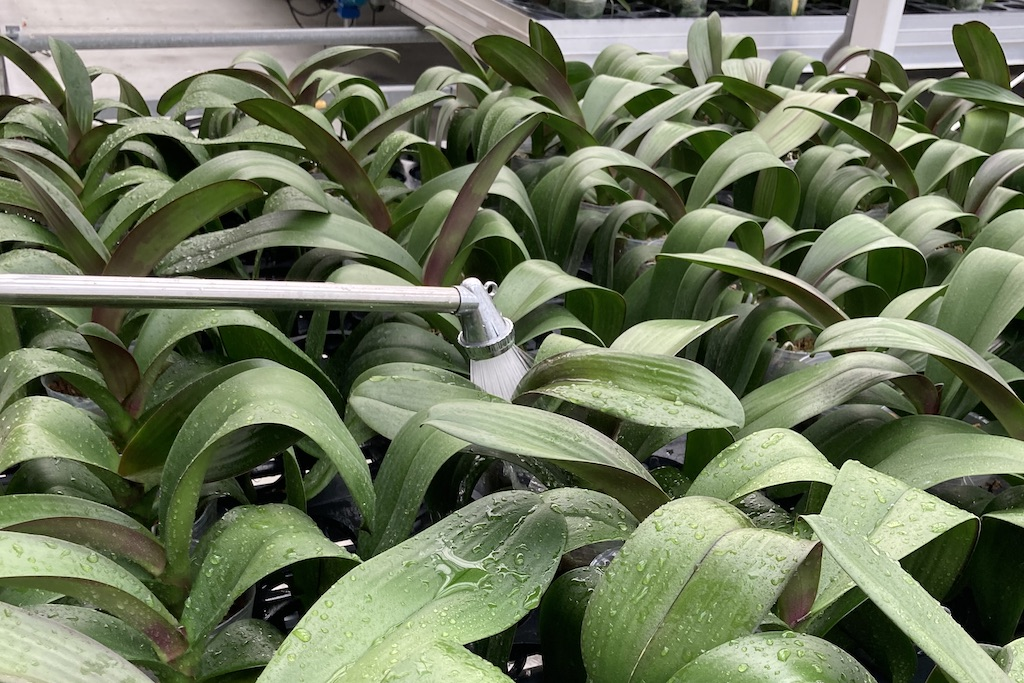
\includegraphics[width=0.7\textwidth]{ch01/HumanWater.jpeg}
    \caption{Farmer is Watering Using Water Jet}
    \label{fig:HumanWater}
\end{figure}

% ===== Check Line V2 2021/08/03

% Using overhead irrigation sys
Recently, most greenhouse companies adopt multiple types of watering machines to solve the lack of laboring resources, including the overhead irrigation system, as shown in Fig.\ref{fig:irrigation_sprinkler}. The overhead irrigation system is cheaper than other systems due to its simple design. Most of the cost comes from the installation of pipes. Besides, by adjusting the inlet valve, the amount of water to plants is controllable. For example, a computer controls the valve to water the whole greenhouse in our cooperative company periodically.

% overhead irrigation sys disadvantage, using gantry
However, the overhead irrigation system will make the whole greenhouse moist, leading to more plant diseases. According to the research about plant diseases from A. Henn, C. Hong and G. Moorman\cite{henn_2016, Plant_Pathogens}, the incidence rate of plants increases with the moisture in the air or the water on leaves. Facing this problem, the cooperative orchid greenhouse has tried another approach, such as the simple watering gantry machine showed in Fig.\ref{fig:old_gantry}. The watering gantry machine is fixed, and there is a set of water sprayers on it. The machine can water plants on the planting bed uniformly by pushing the planting bed and by spreading the water from the water spray. This solution keeps water spread under the gantry so that it decreases the moisture inside the greenhouse.

\begin{figure}[ht]
    \centering
    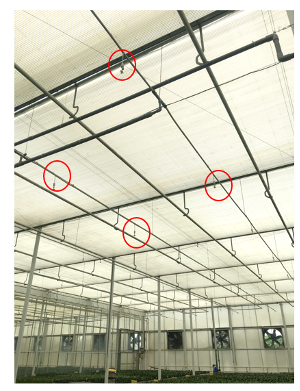
\includegraphics[height=6cm]{ch01/irrigation_sprinkler_1.png}
    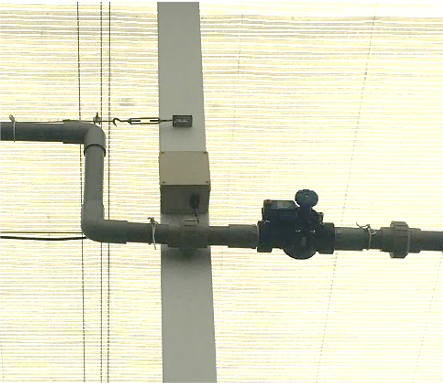
\includegraphics[height=6cm]{ch01/irrigation_sprinkler_2.png}
    \caption{Overhead Irrigation System Installed in Greenhouse}
    \label{fig:irrigation_sprinkler}
\end{figure}

% gantry disadvantage
In spite of preventing the increment of moisture in the greenhouse, the watering gantry machine still suffers some problems. For example, the sprayers installed on the device remain watering both plant roots and leaves. The excessive water accumulation in the root consequently causes the death of plants. Besides, after using the gantry machine, the infiltration on leaves is still not solved, which also increases the incidence rate of plants.

\begin{figure}[ht]
    \centering
    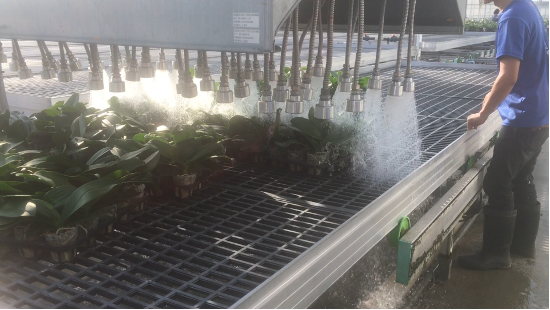
\includegraphics[height=6cm]{ch01/old_gantry_1.png}
    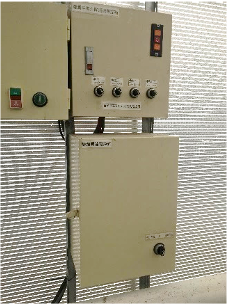
\includegraphics[height=6cm]{ch01/old_gantry_2.png}
    \caption{Traditional Gantry Water Machine}
    \label{fig:old_gantry}
\end{figure}

Until now, a large number of automatic machines cannot solve the difficult problem that a large amount of water remains on the leaves after the orchid seedlings are watered. Additionally, it is not reasonable to avoid the disadvantages of the watering machine by instead adopting human power in large-scale farming. Thus, in recent years, the techniques of computer vision and neural networks have been developed to help resolve many agricultural problems, such as using a convolutional neural network to count the number of seedlings\cite{jausih_2020}. Furthermore, there are also researches of agricultural robots trying to build an automatic system to monitor and control the growth of plants individually. Hence, the research of agricultural robots may be a practical solution to the remaining water problem.